%%%%%%%%%%%%%%%%%%% %%%%%%%%%%%%%%%%%%%%%%
% NIWeek 2014 Poster by T. Reveyrand
% www.microwave.fr
% http://www.microwave.fr/LaTeX.html
% ---------------------------------------
% 
% Original template created by:
% Brian Amberg (baposter@brian-amberg.de)
%
% This template has been downloaded from:
% http://www.LaTeXTemplates.com
%
% License:
% CC BY-NC-SA 3.0 (http://creativecommons.org/licenses/by-nc-sa/3.0/)
%
%%%%%%%%%%%%%%%%%%%%%%%%%%%%%%%%%%%%%%%%%

%----------------------------------------------------------------------------------------
%	PACKAGES AND OTHER DOCUMENT CONFIGURATIONS
%----------------------------------------------------------------------------------------

\documentclass[a0paper,portrait]{baposter}

\usepackage[font=small,labelfont=bf]{caption} % Required for specifying captions to tables and figures
\usepackage{booktabs} % Horizontal rules in tables
\usepackage{relsize} % Used for making text smaller in some places

\usepackage{amsmath,amsfonts,amssymb,amsthm, stmaryrd} % Math packages
\usepackage{eqparbox}

\usepackage{textcomp}
\usepackage{color}
\usepackage{colortbl}
\usepackage{multirow}
\usepackage{amsmath}
\DeclareMathOperator*{\argmax}{arg\,max}

\graphicspath{{figures/}} % Directory in which figures are stored

 \definecolor{bordercol}{RGB}{40,40,40} % Border color of content boxes
 \definecolor{headercol1}{RGB}{186,215,230} % Background color for the header in the content boxes (left side)
 \definecolor{headercol2}{RGB}{120,120,120} % Background color for the header in the content boxes (right side)
 \definecolor{headerfontcol}{RGB}{0,0,0} % Text color for the header text in the content boxes
 \definecolor{boxcolor}{RGB}{210,235,250} % Background color for the content in the content boxes
% \definecolor{boxcolor}{RGB}{255,255,255}
 
 \usepackage{algorithm}
\usepackage[noend]{algpseudocode} 

\usepackage[all,pdftex]{xy}
% For faster compilation. Entries must be wrapped in curly braces!
\CompileMatrices 
\xyoption{v2}
\xyoption{curve}
\xyoption{2cell}
\SelectTips{cm}{}  % Tips (of arrows) are in accordance with Computer Modern
\UseAllTwocells
%\SilentMatrices
\def\labelstyle{\textstyle}
\def\twocellstyle{\textstyle}

\newcommand{\bu}{\mathbf{u}}
\newcommand{\bv}{\mathbf{v}}
\newcommand{\bw}{\mathbf{w}}

% define some signal names as abbreviations
\newcommand{\throttle}{\mathit{throttle}}
\newcommand{\brake}{\mathit{brake}}
\newcommand{\speed}{\mathit{speed}}
\newcommand{\rpm}{\mathit{rpm}}
\newcommand{\gear}{\mathit{gear}}
\newcommand{\AF}{\mathit{AF}}
\newcommand{\AFref}{\mathit{AF}_\text{ref}}

\newcommand{\DiaOp}[1]{\Diamond_{#1}}
\newcommand{\BoxOp}[1]{\square_{#1}}

\newcommand{\yes}{20*}
\newcommand{\no}{0*}

\newcommand{\Falsify}{\mathsf{Falsify}}
\newcommand{\STL}{\textbf{STL}}
\newcommand{\Rpos}{\R_{>0}}
\newcommand{\R}{{\mathbb{R}}}
\newcommand{\N}{{\mathbb{N}}}


\DeclareMathOperator*{\argmin}{arg\,min}

\newcommand{\sem}[1]{\llbracket #1 \rrbracket} 

\begin{document}

\background{ % Set the background to an image (background.pdf)
\begin{tikzpicture}[remember picture,overlay]
\draw (current page.north west)+(-2em,2em) node[anchor=north west]
{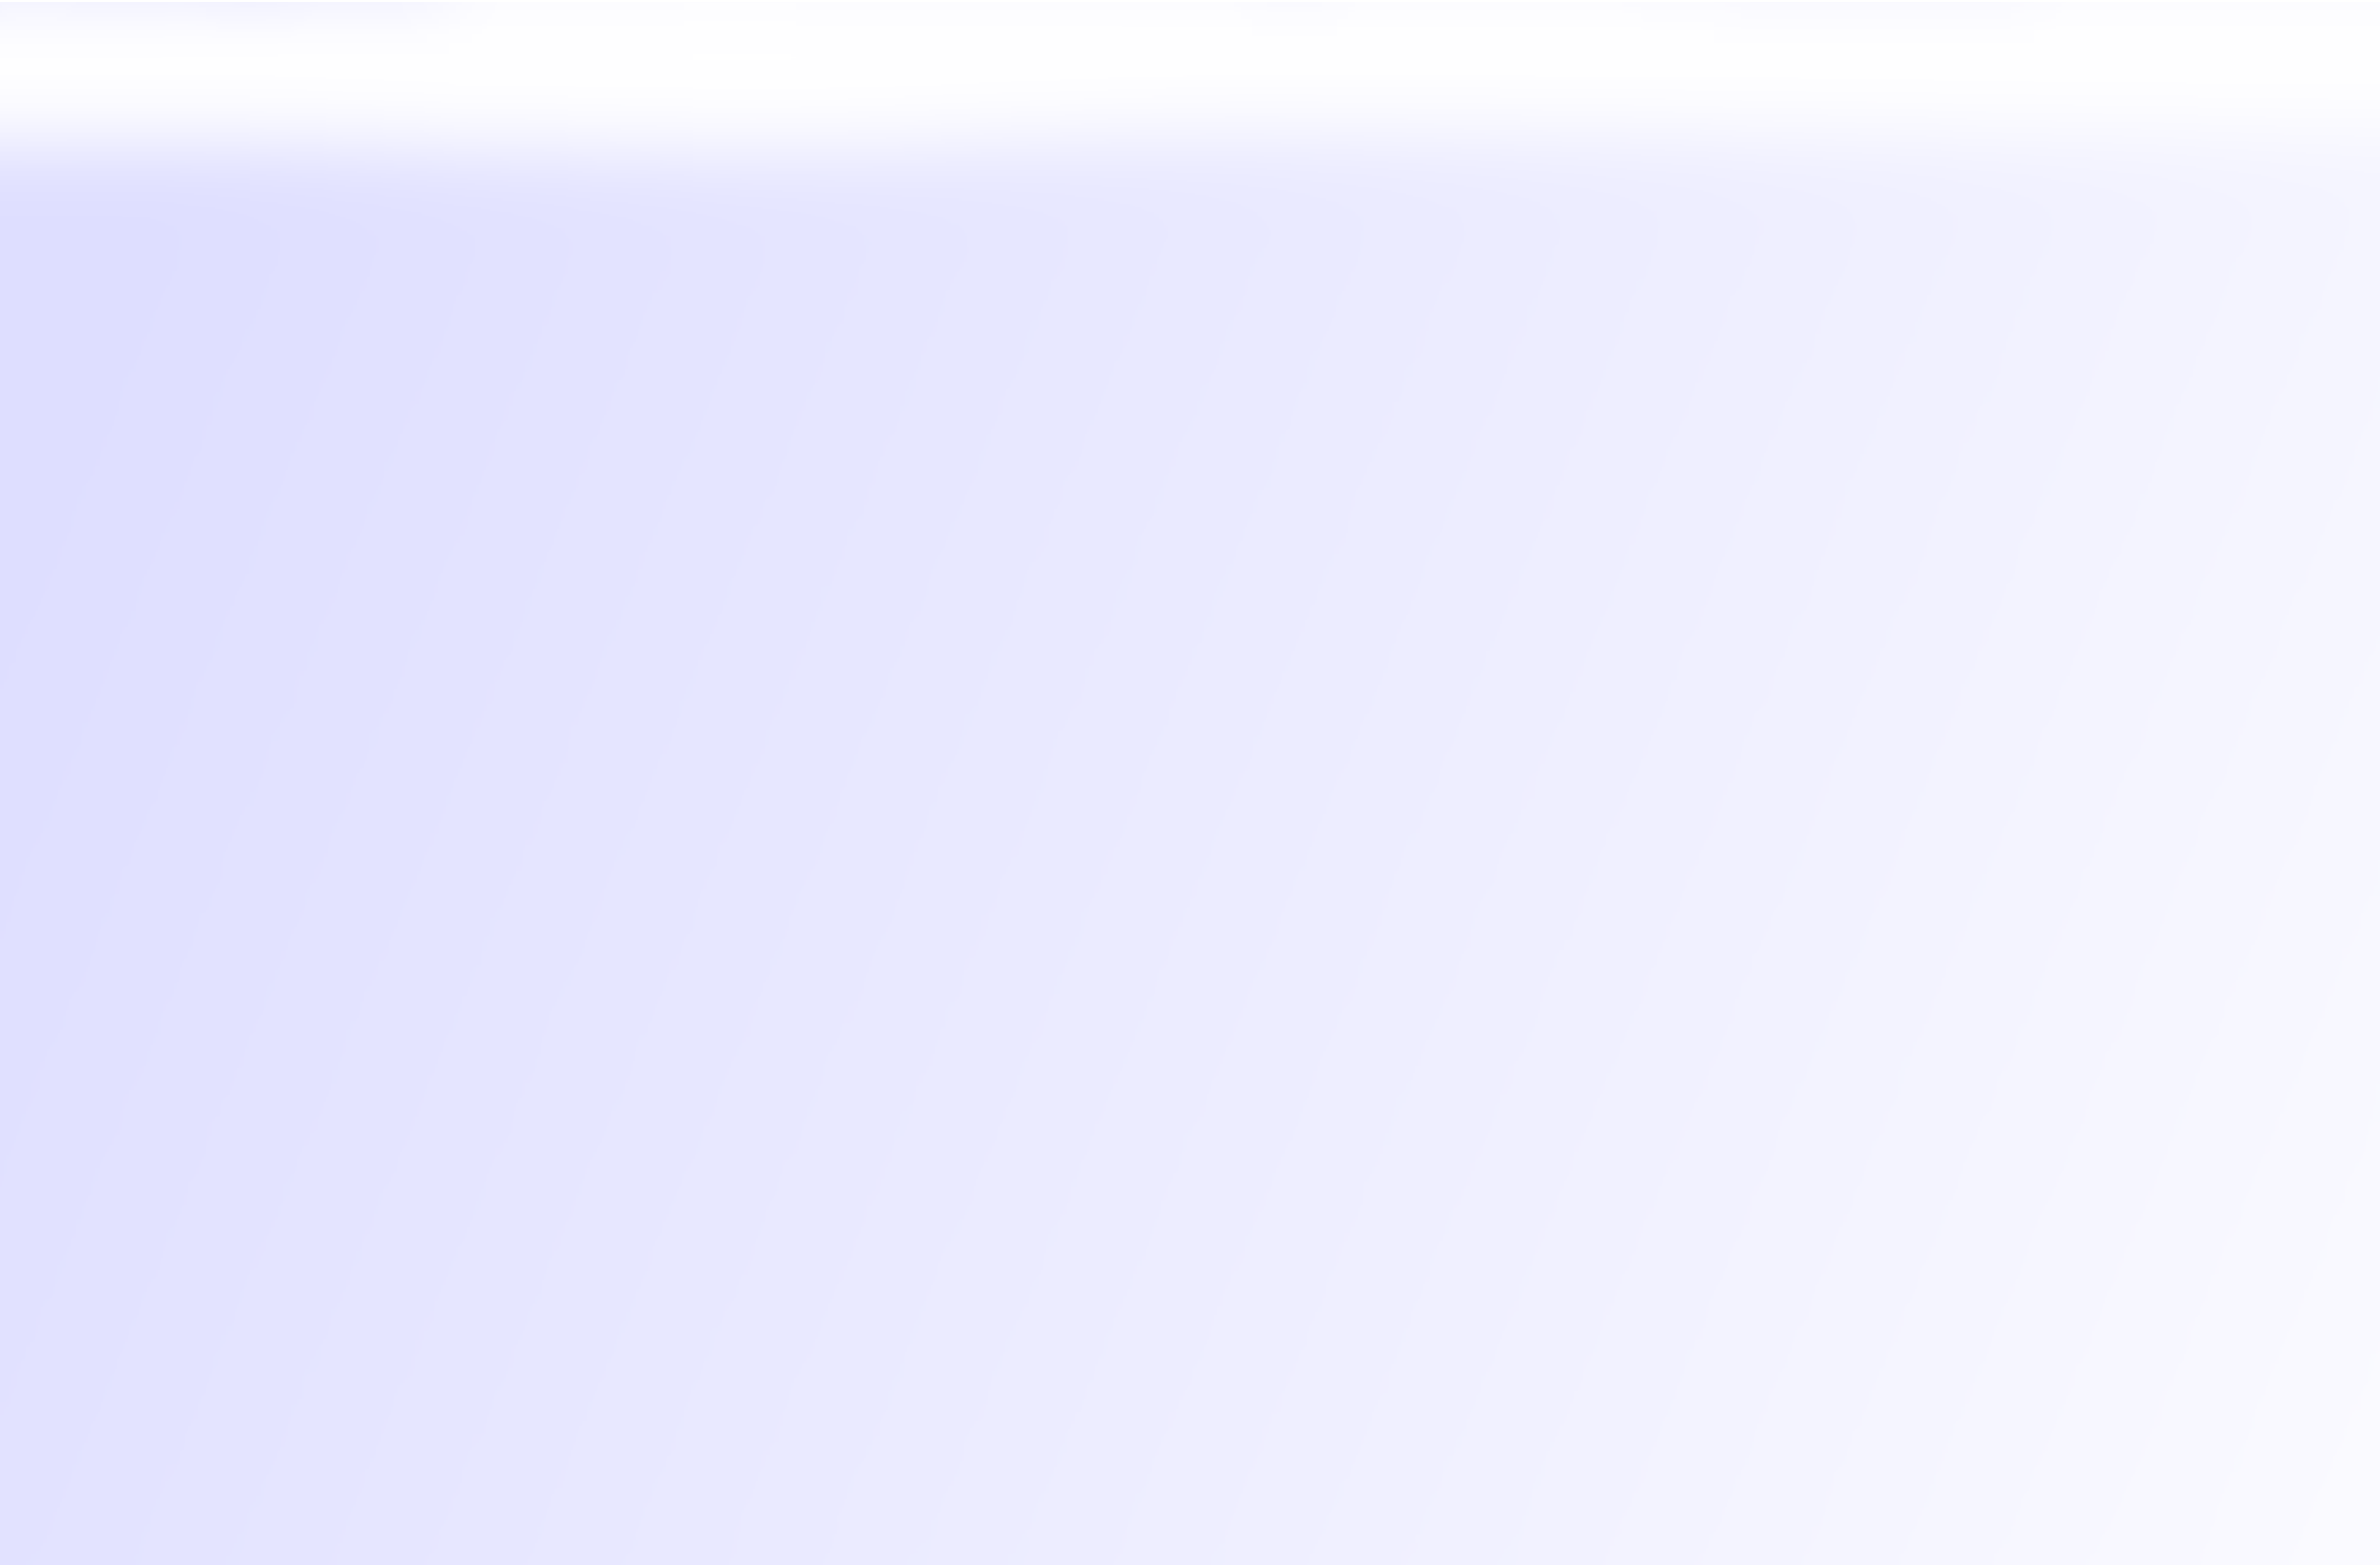
\includegraphics[height=1.1\textheight]{background}};
\end{tikzpicture}
}

\begin{poster}{
grid=false,
borderColor=bordercol, % Border color of content boxes
headerColorOne=headercol1, % Background color for the header in the content boxes (left side)
headerColorTwo=headercol2, % Background color for the header in the content boxes (right side)
headerFontColor=headerfontcol, % Text color for the header text in the content boxes
boxColorOne=boxcolor, % Background color for the content in the content boxes
headershape=roundedright, % Specify the rounded corner in the content box headers
headerfont=\Large\sf\bf, % Font modifiers for the text in the content box headers
textborder=rectangle,
background=user,
headerborder=open, % Change to closed for a line under the content box headers
boxshade=plain
}
{
\includegraphics[scale=0.2]{erato.png}}
%
%----------------------------------------------------------------------------------------
%	TITLE AND AUTHOR NAME
%----------------------------------------------------------------------------------------
%
{\huge    {Stochastic Optimization based Hybrid System Falsification} } % Poster title
{\vspace{0.3em} \smaller Zhenya Zhang  \\  % Author names
   \smaller \it{zhangzy@nii.ac.jp} \\
\smaller \it {National Institute of Informatics, Tokyo, Japan}\\ \it{The Graduate University for Advanced Studies (SOKENDAI), Hayama, Japan} } % Author email addresses
%{\includegraphics[scale=0.45]{NI.jpg}} % University/lab logo

%----------------------------------------------------------------------------------------
%	INTRODUCTION
%----------------------------------------------------------------------------------------
\headerbox{Quality assurance of Cyber-Physical Systems}{name=introduction,column=0,row=0, span=3}{

\begin{minipage}[h]{0.4\textwidth}
\centering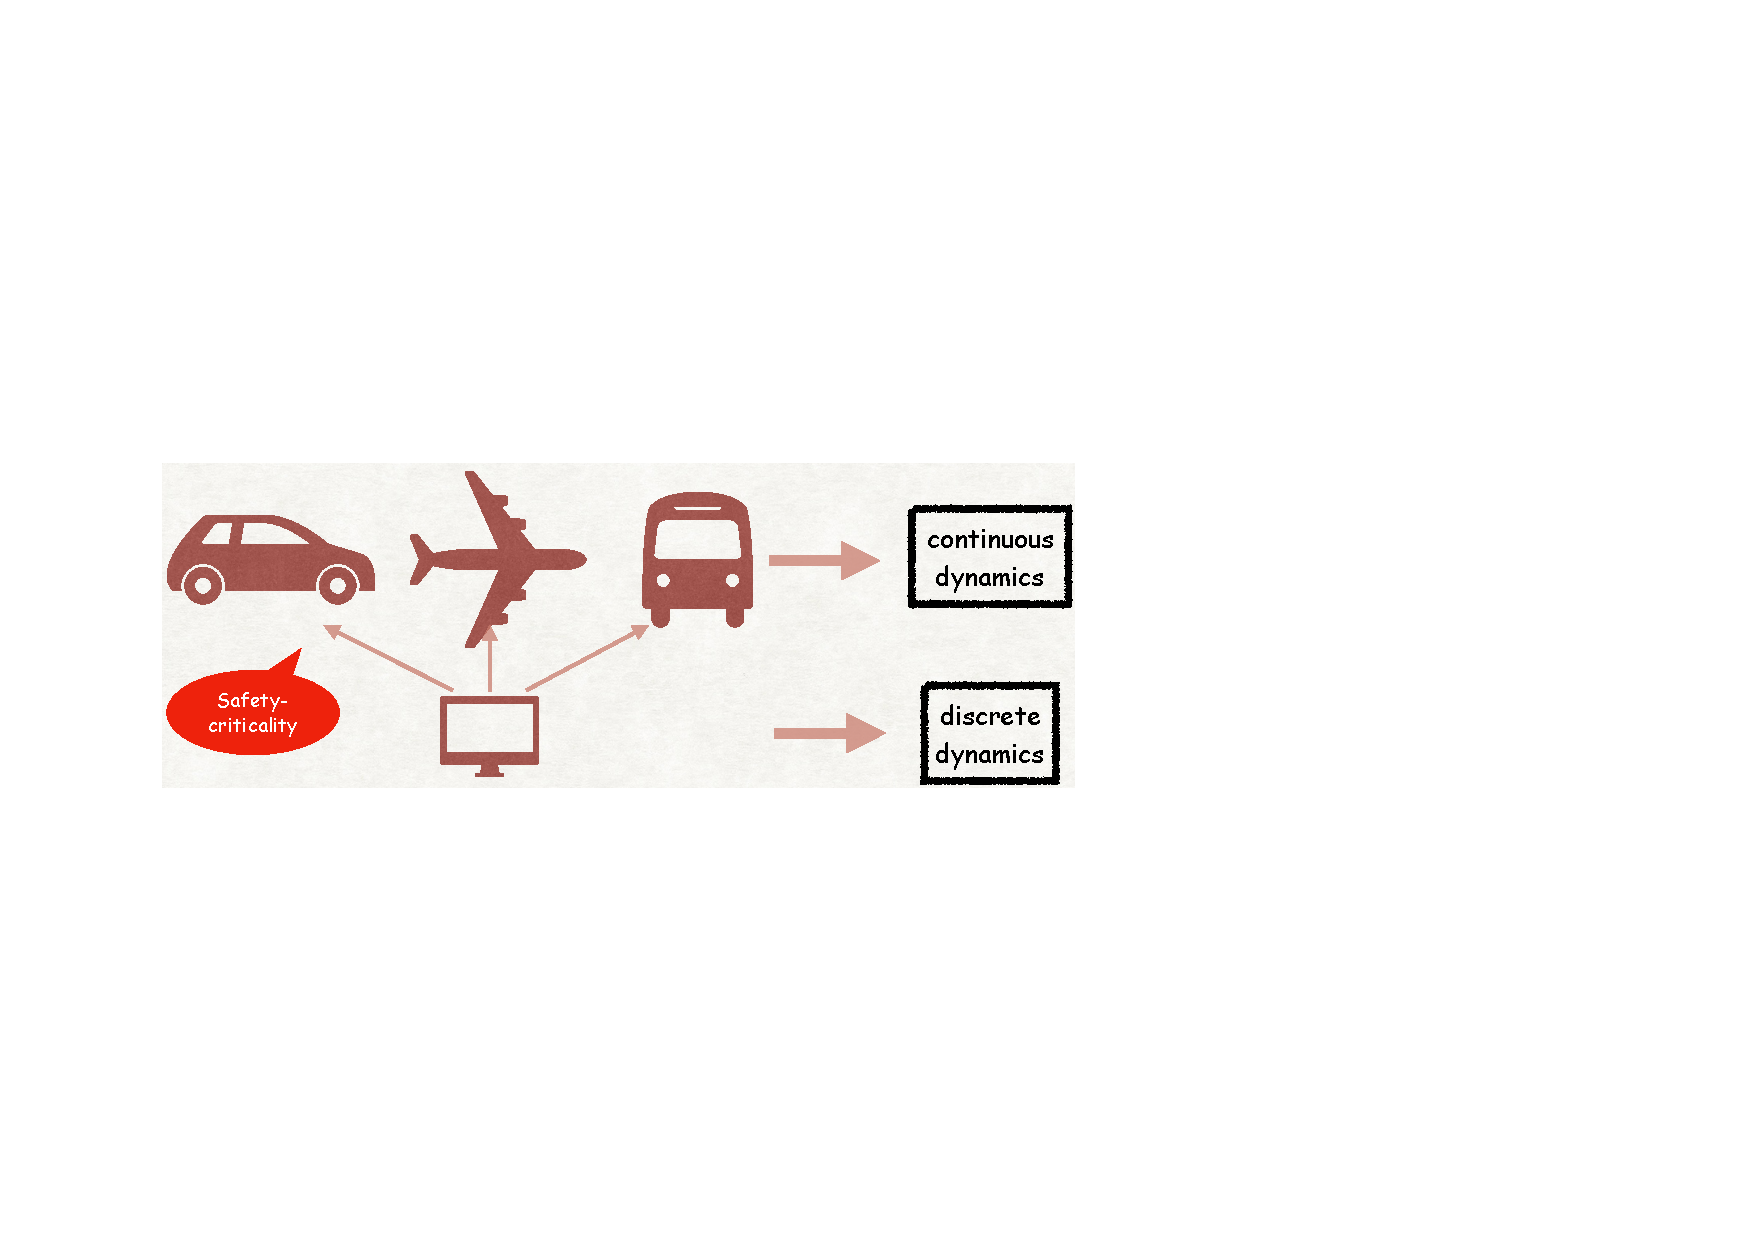
\includegraphics[scale=0.55]{figures/cps.pdf}
\end{minipage}
\begin{minipage}[h]{0.6\textwidth}
Why falsification?
\begin{itemize}
\vspace{-0.8em}
\item Verification based on system exploration is infeasible because of infinite state space.
\vspace{-0.8em}
\item Testing which aims at a counterexample refuting the specification is more suited.
\end{itemize}
\vspace{-0.8em}
The advantages of falsification:
\begin{itemize}
\vspace{-0.8em}
\item Aims at one counterexample, much easier and more feasible than verification.
\vspace{-0.8em}
\item Be able to handle black-box model, no need to know the dynamics.
\vspace{-0.8em}
\item Rely on optimization techniques, more intelligent than random sampling.
\end{itemize}
\end{minipage}


}


%----------------------------------------------------------------------------------------
%	CALIBRATION
%----------------------------------------------------------------------------------------
\headerbox{Falsification problem}{name=relwork, column=0, below=introduction}{

Falsification problem is defined as follows:
    \begin{itemize}
    \item{\textbf{Given:}} 
      a \emph{Simulink} model $\mathcal{M}$ or other black box, and
      a \emph{specification} $\varphi$ in Signal Temporal Logic (STL)

    \item{\textbf{Answer:}} 
      \emph{error input}, i.e., an input signal $\bu$ such
      that the corresponding output $\mathcal{M}(\bu)$ violates $\varphi$ 
    \end{itemize}
\begin{minipage}{0.4\textwidth}
\centering
  \begin{math} 
 \hspace{2em} \xymatrix@1@+2.5em{
   {}
     \ar[r]^-{\bu}
   &
   {  \quad\xybox{ *++++[F]{\mathcal{M}} }}
     \ar[r]^-{\mathcal{M}(\bu)}_-{\not\models\varphi \; ?}
   &
   {}
   }
  \end{math}
 \end{minipage}


}




\headerbox{Signal Temporal Logic (STL)}{name=optsolver, column=0, below=relwork}{

%\quad  $\bullet \quad\Box~(\speed < 120)$

STL is used for formalizing system requirements, like safety or comfort concerns 

E.g., $\varphi \equiv \Box_{[0, 30]}(\speed[t] < 120)$

\begin{tabular}{c|c|c}
%\hline
 signal $\bw$  &$\bw\models\varphi$
 & $\sem{\bw,\varphi}$
\\ \hline
 %Boolean\\satisfaction
 \begin{minipage}{0.4\textwidth}\vspace{+0.2em}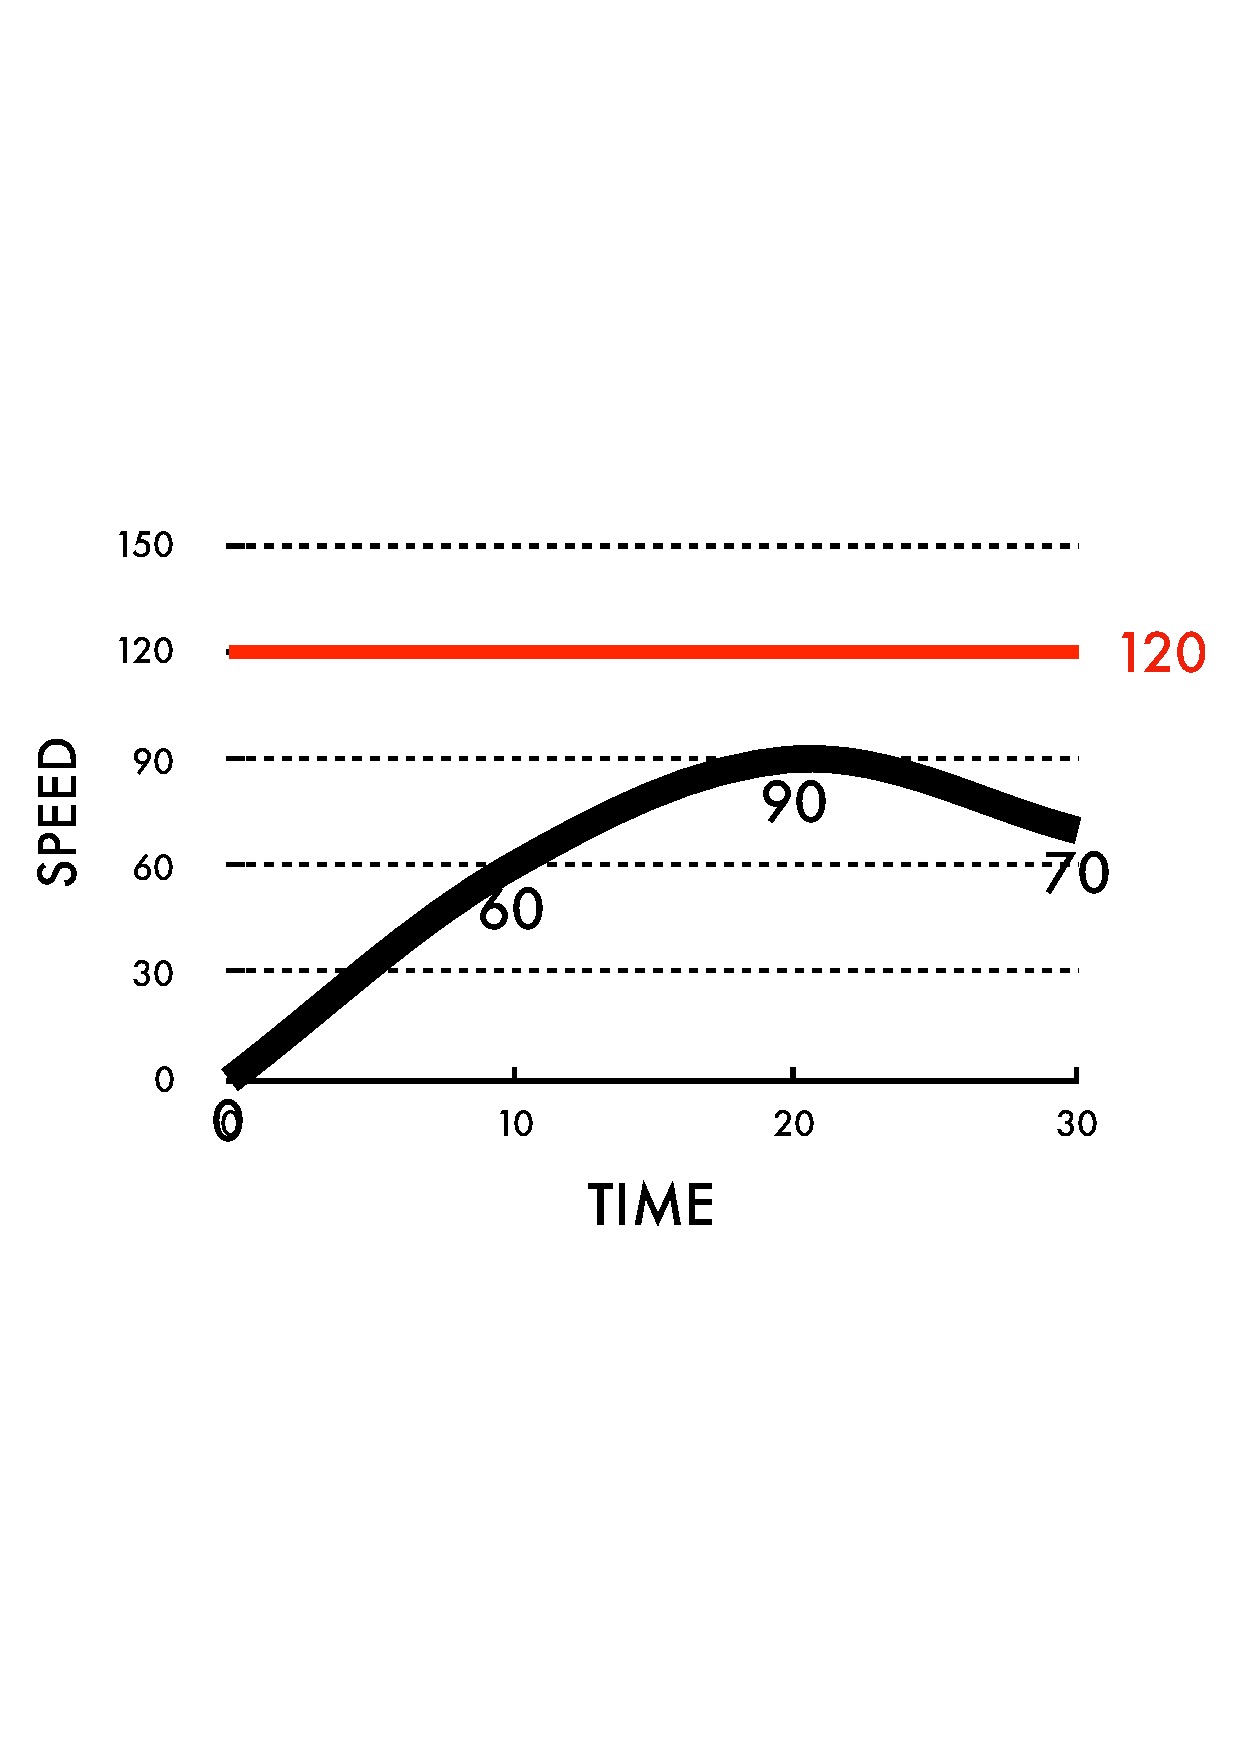
\includegraphics[width=0.99\textwidth]{figures/stleg1.pdf} \end{minipage}\vspace{+0.2em}
& TRUE & 30  \\ \hline
%quantitative\\robustness
 \begin{minipage}{0.4\textwidth}\vspace{+0.2em}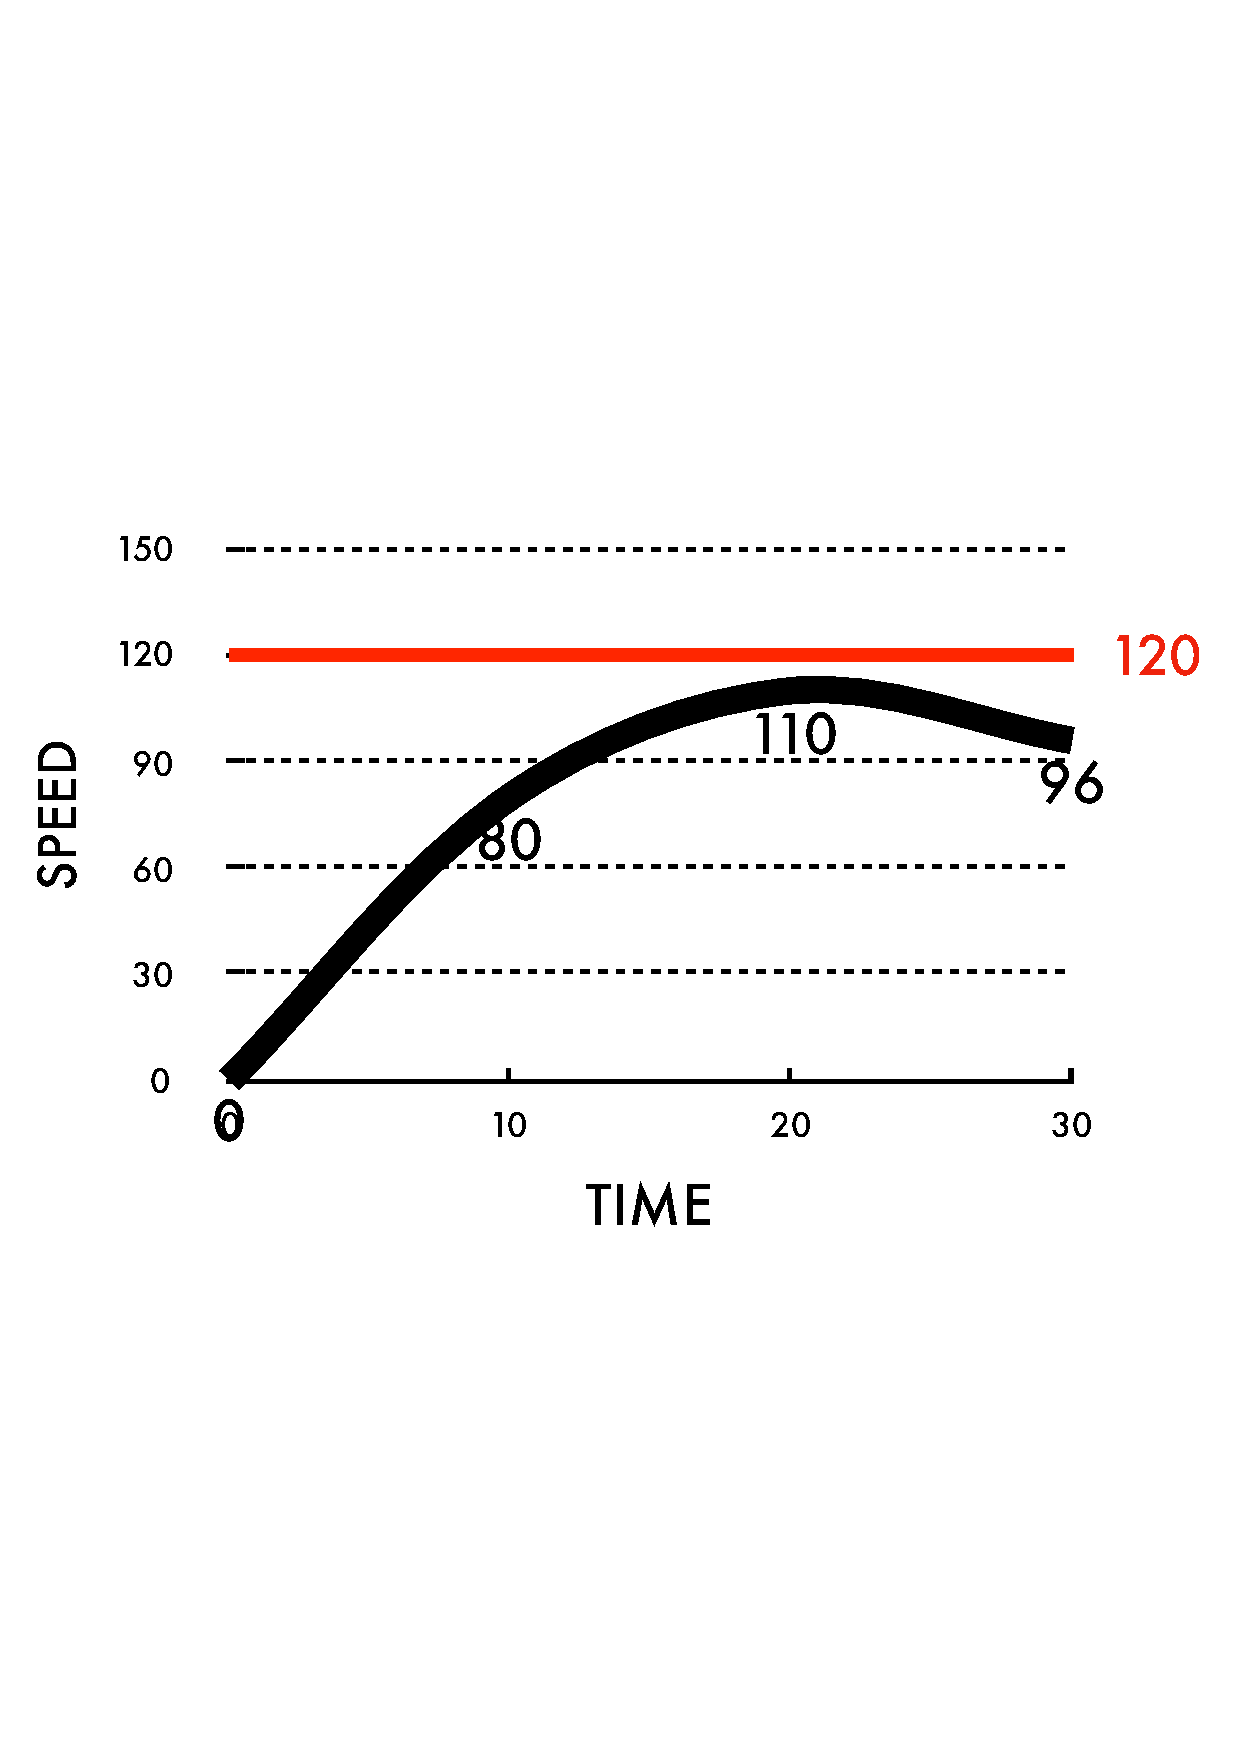
\includegraphics[width=0.99\textwidth]{figures/stleg2.pdf} \end{minipage}  \vspace{+0.2em}
& TRUE & 10 \\ \hline
\begin{minipage}{0.4\textwidth}\vspace{+0.2em}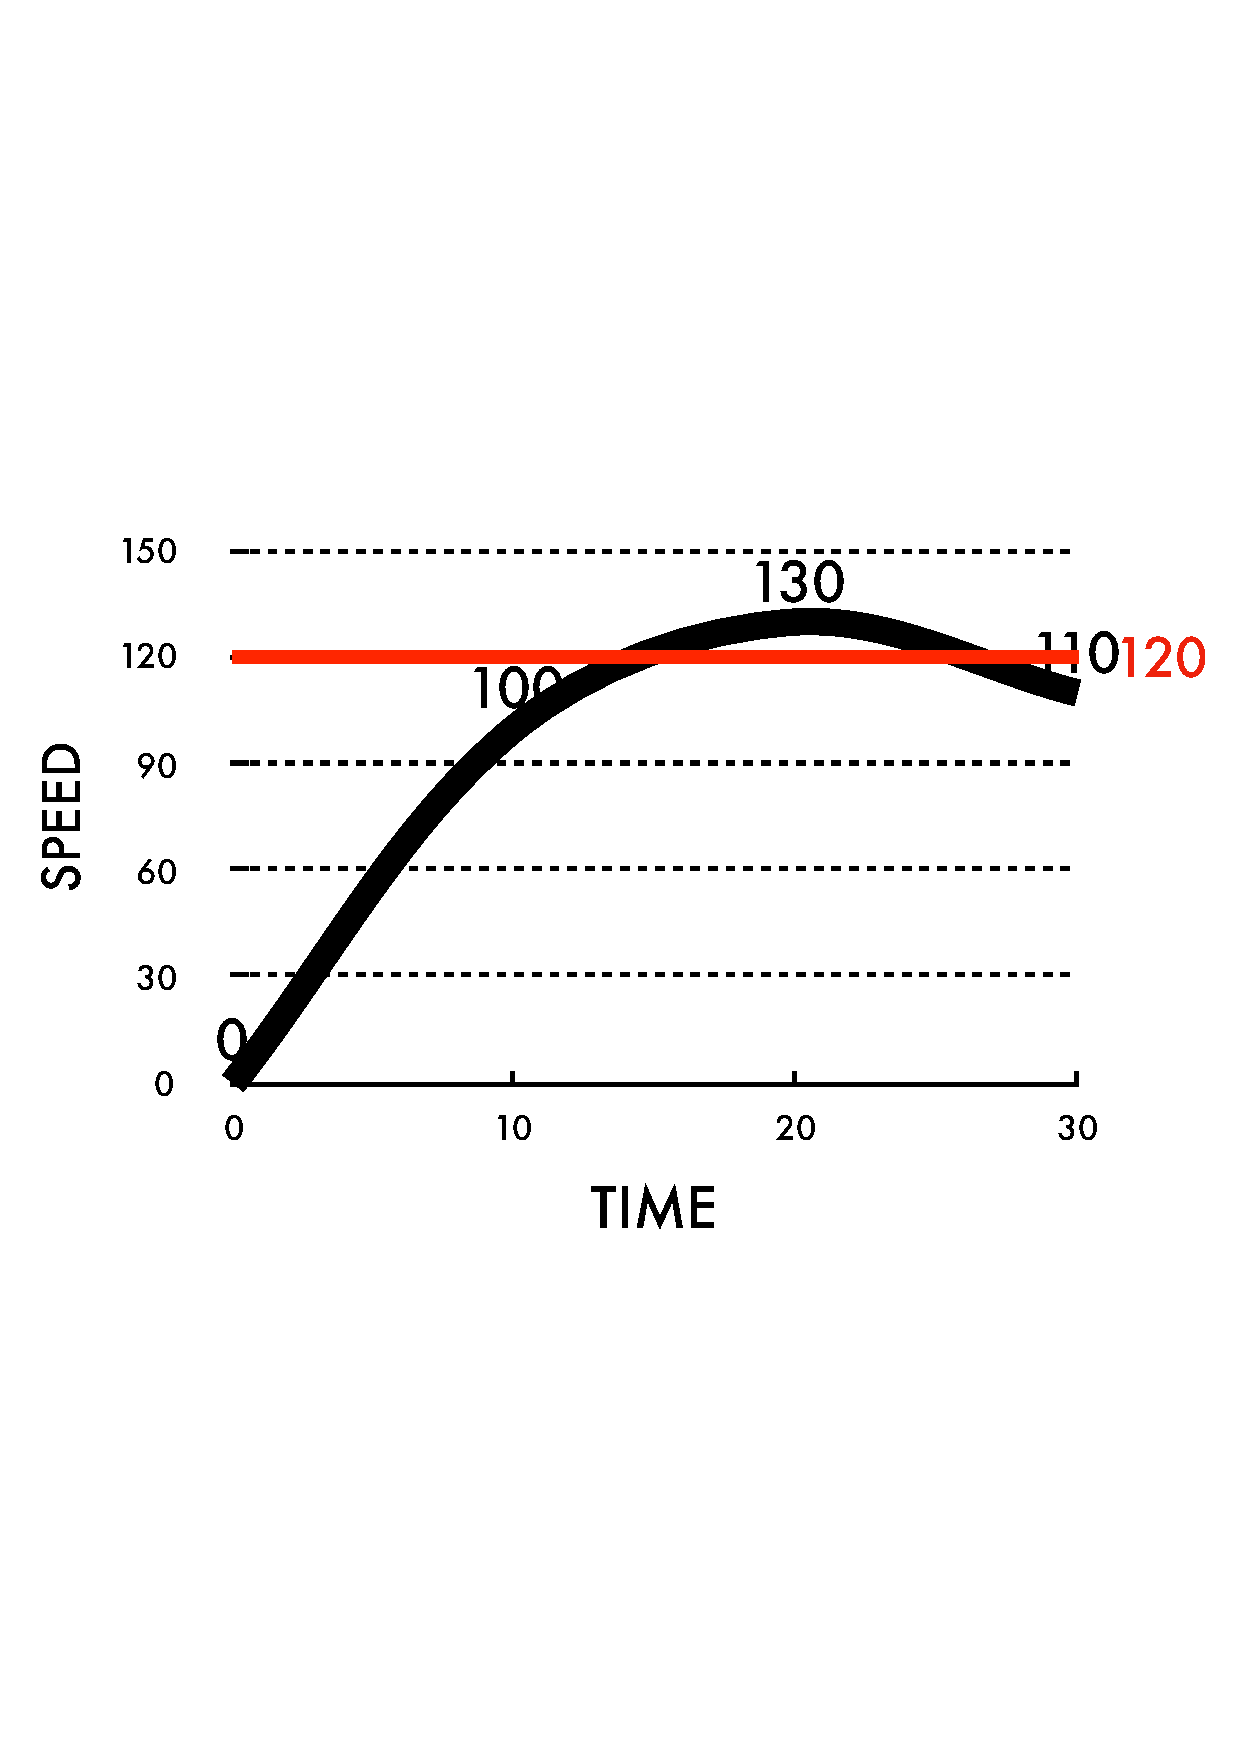
\includegraphics[width=0.99\textwidth]{figures/stleg3.pdf} \end{minipage}\vspace{+0.2em}  
& FALSE & -10 

%\\ \hline
\end{tabular}


  
}

\headerbox{Optimization approach}{name=opt, column=0, below=optsolver}{

%\begin{itemize}
Objective function: 
\vspace{-0.5em}
$$\min_{\bu}\sem{\mathcal{M}(\bu), \varphi}$$\vspace{-2em}

Constraints:
\begin{itemize}
\vspace{-0.8em}
\item $\bu$ is bounded
\vspace{-0.8em}
\item Constraints from domain knowledge.
\end{itemize}

}

\headerbox{``Hill-climbing'' Optimization}{name=hillclimbing, column=0, below=opt}{
\centering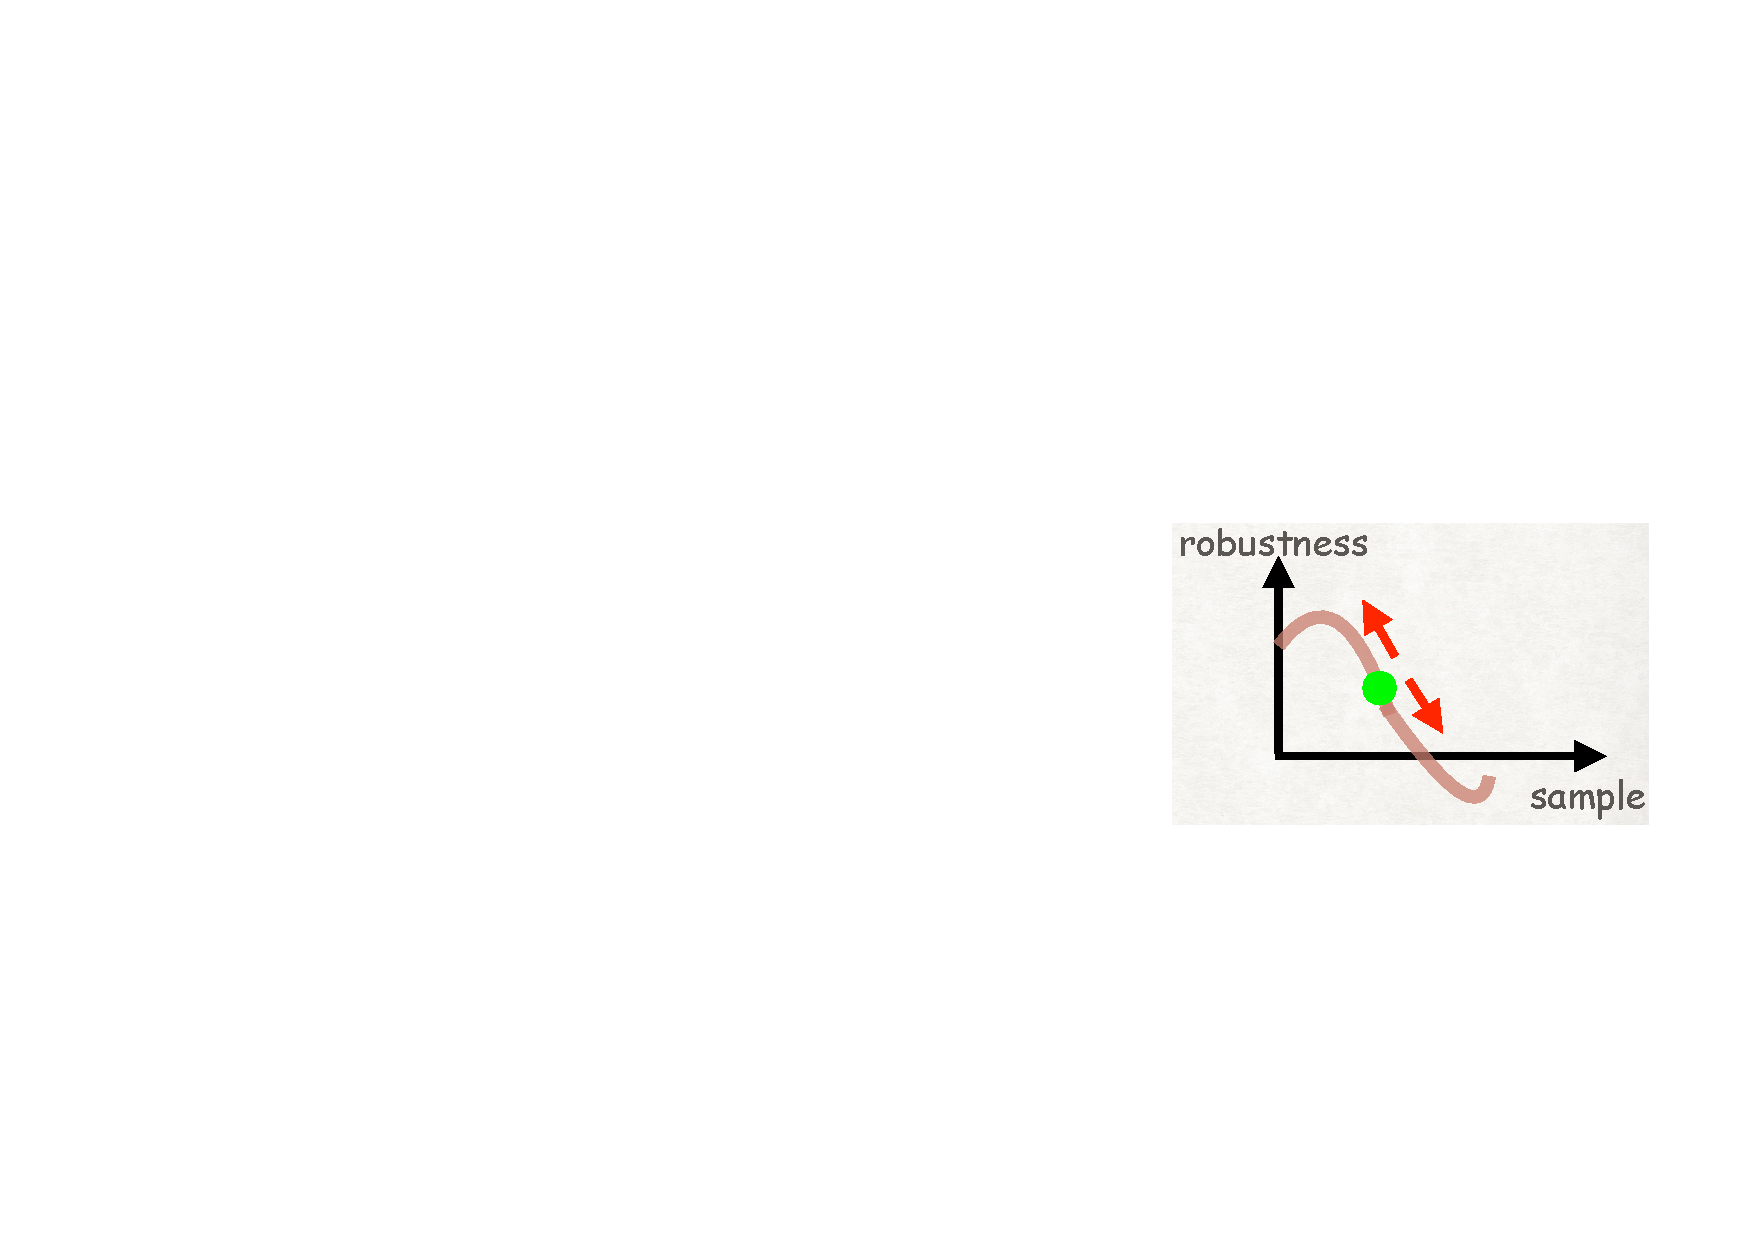
\includegraphics[scale=0.45]{figures/hill-climbing.pdf}

\begin{itemize}
\vspace{-0.8em}
\item Make use of the history sampling.
\vspace{-0.8em}
\item Derivative free.
\vspace{-0.8em}
\item Successful applications:
\begin{itemize}
\vspace{-0.6em}
\item Breach (CMA-ES, NM, etc.)
\vspace{-0.6em}
\item S-TaLiRo (SA, etc.)
\end{itemize}
\end{itemize}
}


%----------------------------------------------------------------------------------------
%	OTHER INSTRUMENTATION
%----------------------------------------------------------------------------------------
\headerbox{Work 1: Monte Carlo Tree Search for Global Optimum}{name=algorithm,span=2,column=1,row=1, below=introduction}{ % To reduce this block to 1 column width, remove 'span=2'
\begin{minipage}[h]{0.24\textwidth}
\centering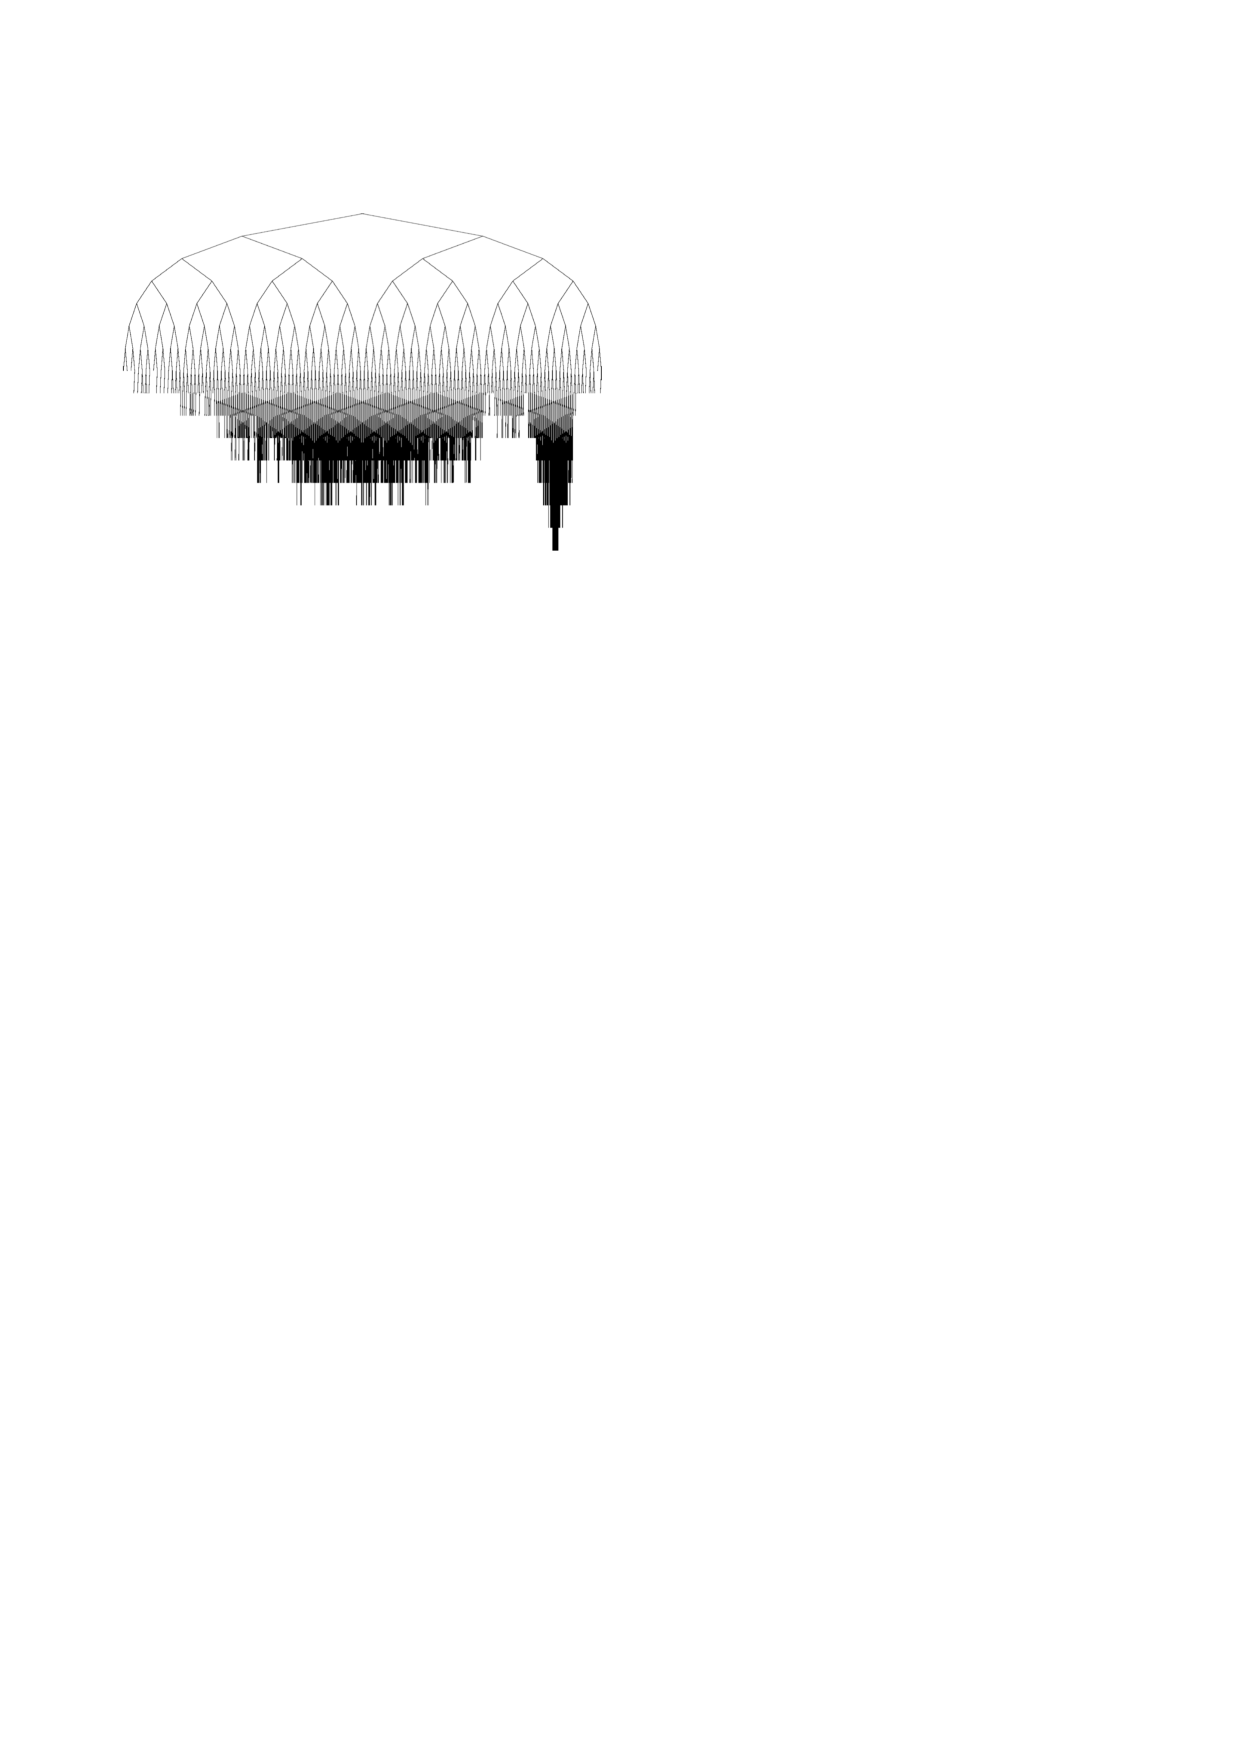
\includegraphics[scale=0.4]{figures/mcts.pdf}
\end{minipage}
\begin{minipage}[h]{0.76\textwidth}
\centering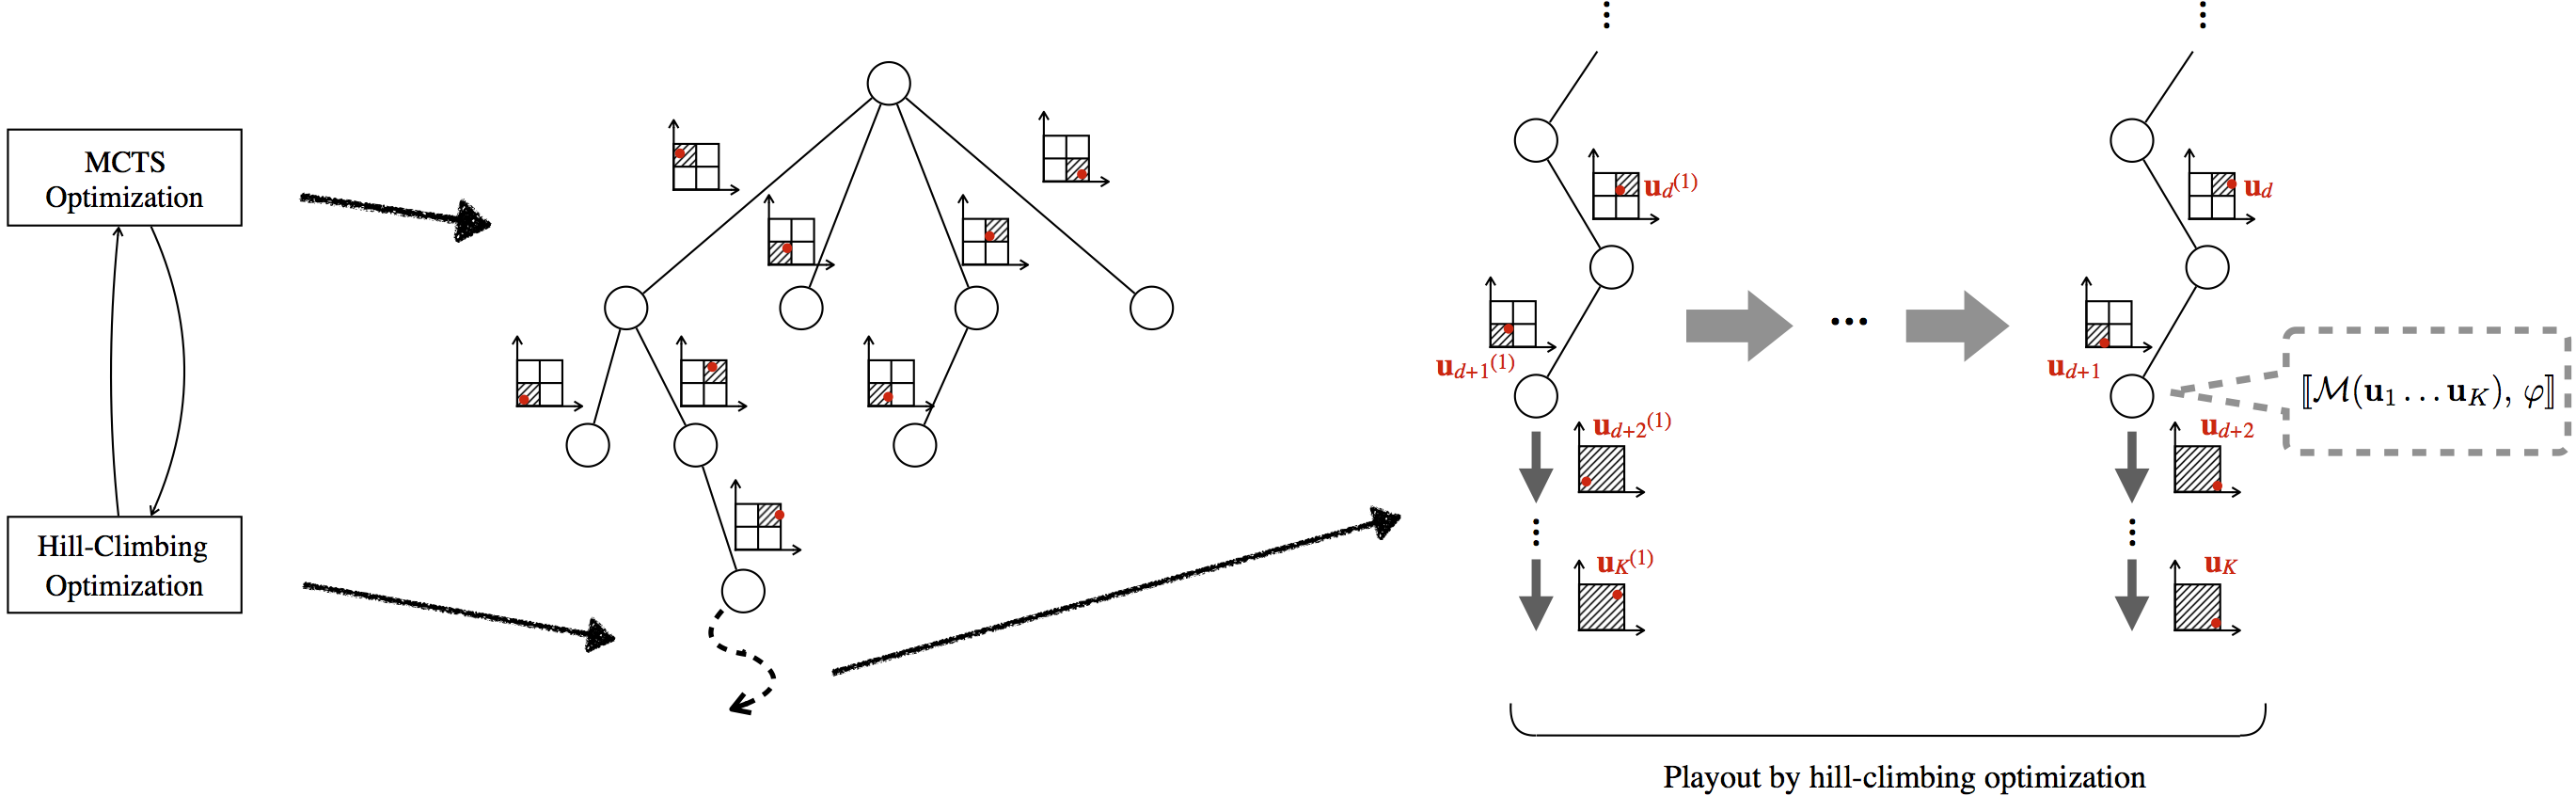
\includegraphics[scale=.1]{figures/algorithm.png}
\end{minipage}




\begin{itemize}
\vspace{-0.8em}
\item Time-staging. Divide the time bound into $K$ intervals to find a sequence $\bu_{1},\dotsc,\bu_{K}$.


\vspace{-0.8em}
\item Node expansion. Use a \emph{partitioning} of the input space $I_{1}\times\cdots\times I_{M}$ as the children set $A$.
\vspace{-0.8em}

\item Child selection. Define that $reward = 1-\frac{R(wa)}{\max_{w'\in\mathcal{T}}R(w')}$, and apply UCB1 algorithm $\argmax_{a\in A} \left(reward + c\sqrt{\frac{2\ln N(w)}{N(wa)}}\right)$ to select the best child.
\vspace{-0.8em}

\item Simulation. Apply optimization solvers in the selected sub-region sequence with time budget.

\vspace{-0.8em}


\item Backpropagation. Update the reward of parent if the newly computed reward is better.


\end{itemize}


}


%----------------------------------------------------------------------------------------
%	MIXER vs. SAMPLERS
%----------------------------------------------------------------------------------------
\headerbox{Work 2: Multi-armed Bandits for Boolean Connectives}{name=autotrans, span=2, column=1, row=1, below=algorithm}{
\begin{minipage}[h]{0.35\textwidth}
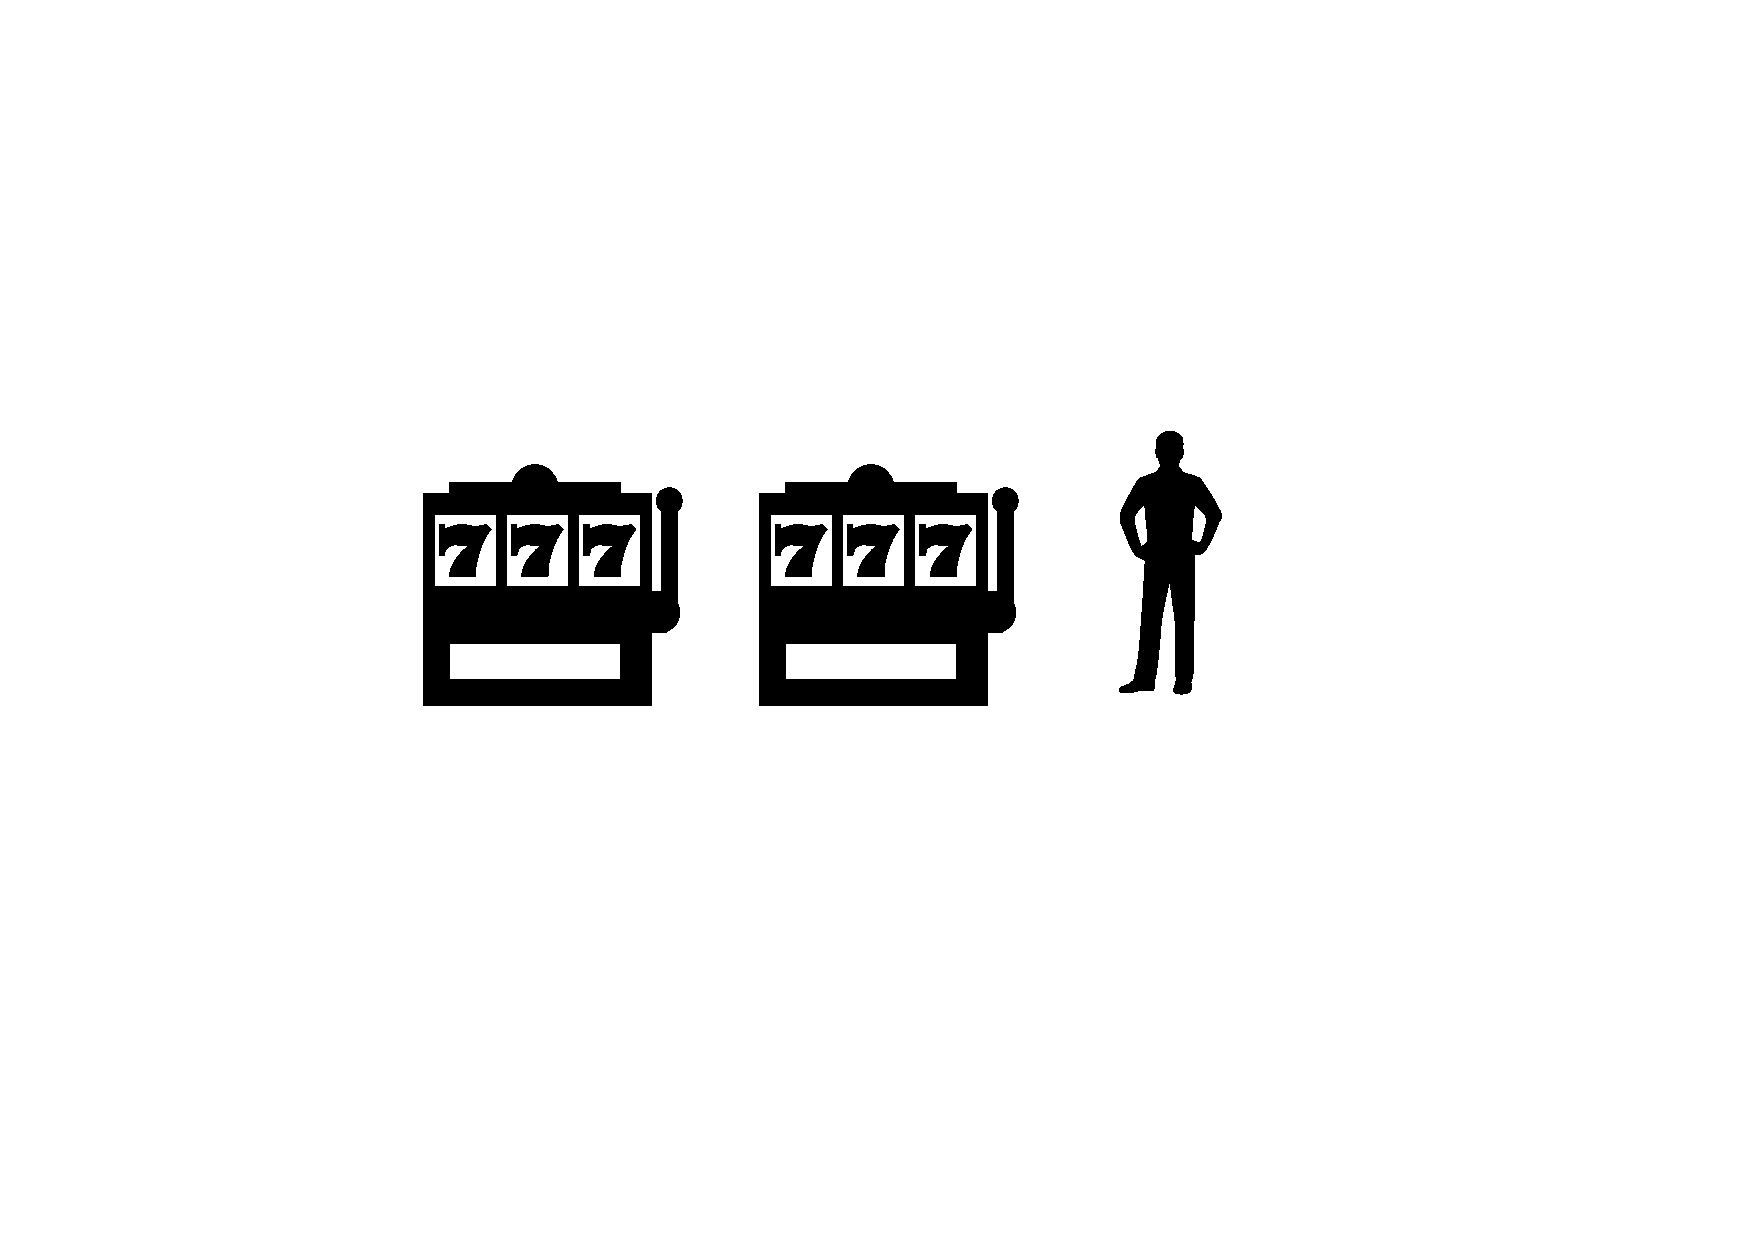
\includegraphics[scale=0.35]{figures/mab.pdf}
\end{minipage}
\begin{minipage}[h]{0.65\textwidth}
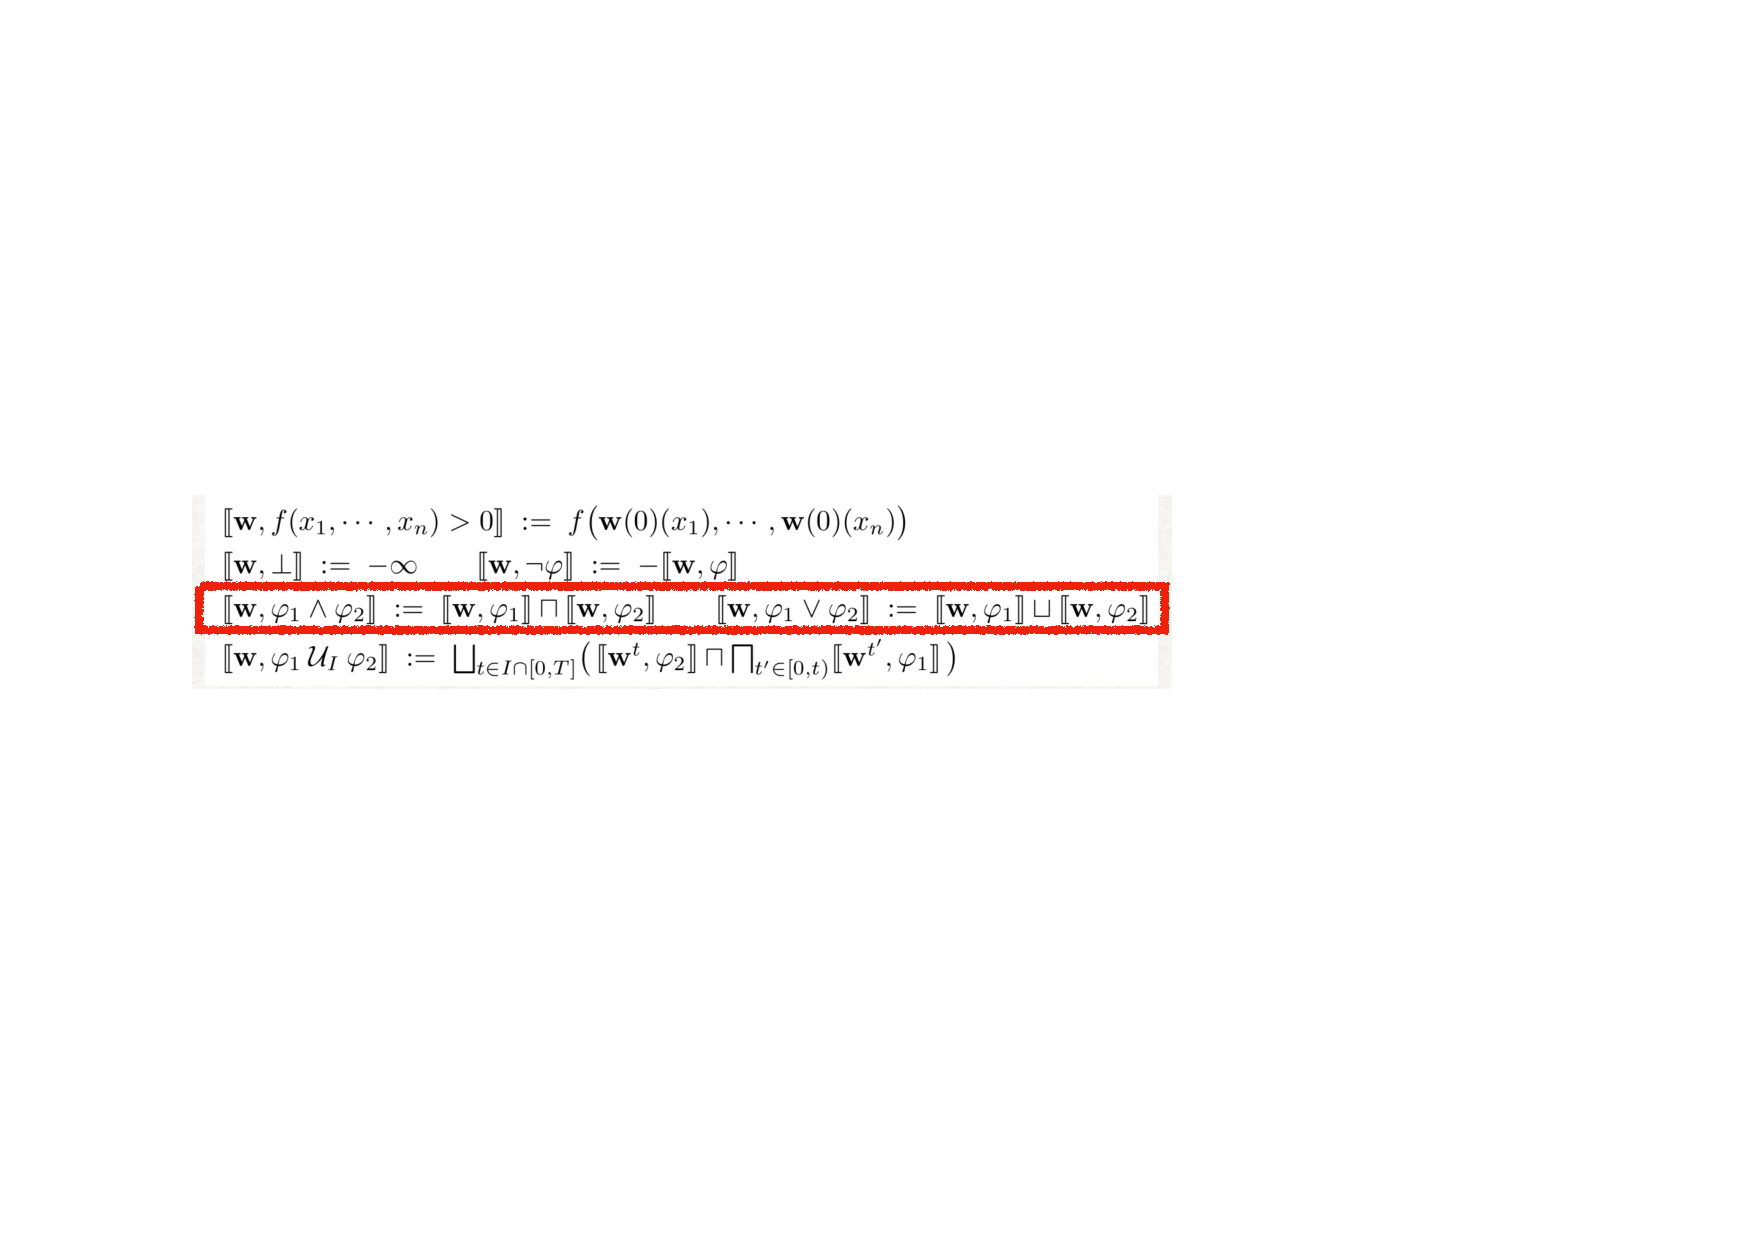
\includegraphics[scale=0.54]{figures/stlsemantics.pdf}
\end{minipage}

\begin{minipage}[h]{0.45\textwidth}
  To handle conjunctive $\varphi\equiv \varphi_1\land \varphi_2$

 \begin{itemize}
 \vspace{-0.8em}
 \item It suffices to falsify either $\sem{\mathcal{M}(\bu), \varphi_1}$ or $\sem{\mathcal{M}(\bu), \varphi_2}$
 \vspace{-0.8em}
 \item Apply algorithms for MAB, such as UCB1, $\epsilon$-greedy, to alternatively optimize $\sem{\mathcal{M}(\bu), \varphi_1}$ and $\sem{\mathcal{M}(\bu), \varphi_2}$
 \vspace{-0.8em}
 \item The reward is defined as 

 $\displaystyle
 \frac{ \mathsf{max\text{-}rb}({i},k-1)
 - \mathsf{last\text{-}rb}({i},k-1)}{\mathsf{max\text{-}rb}({i},k-1)}$





 \end{itemize}
\end{minipage}
\begin{minipage}[h]{0.48\textwidth}
To handle disjunctive $\varphi\equiv\varphi_1\lor \varphi_2$:
\begin{itemize}
 \vspace{-0.8em}
\item In this case, it is not sufficient to falsify only $\sem{\mathcal{M}(\bu), \varphi_1}$ or $\sem{\mathcal{M}(\bu), \varphi_2}$
  \vspace{-0.8em}
 \item $\sem{\mathcal{M}(\bu), \varphi_i}_S$ is defined as\\
$\mathcal{S}=\bigl\{\,t\in I\cap [0,T]\,\big|\, \sem{\mathcal{M}(\bu^{t}), \varphi_{\overline{i}}}<0\,\bigr\}$
 \vspace{-0.8em}
 \item Similarly, we apply MAB algorithms to alternatively optimize $\sem{\mathcal{M}(\bu), \varphi_1}_S$ and $\sem{\mathcal{M}(\bu), \varphi_2}_S$
 \vspace{-0.8em}
 \item The reward is defined accordingly.
\end{itemize}
\end{minipage}

%\end{small}
}


%----------------------------------------------------------------------------------------
%	MEASUREMENT SETUP
%----------------------------------------------------------------------------------------



%----------------------------------------------------------------------------------------
%	CONCLUSION
%----------------------------------------------------------------------------------------
\headerbox{Case Study 1}{name=conclusion1,column=1,below=autotrans,span=1}{

{${\varphi\equiv \Box_{[0,30]}(\rpm < 4770 \lor \Box_{[0,1]}(\rpm > 600))}$}

\textbf{Comment} The property states that when the RPM is over 4770, it should not drop drastically to 600 within 1 second.

\textbf{Comparison with Breach}

\vspace{-0.5em}
\begin{center}
\begin{tabular}{ccc}
\hline
       & FR   & time (s) \\ \hline
Breach & 3/10 & 75.5     \\ \hline
P.A.    & 9/10 & 384.4   \\\hline
\end{tabular}
\end{center}

\textbf{Discussion} For the falsification rate, our proposed approach is better than Breach; 
for the time consumption, our approach takes longer than Breach, which is reasonable since MCTS
takes more efforts on exploration. 


}
\headerbox{Case Study 2}{name=conclusion,column=2,below=autotrans,span=1}{

{${\varphi\equiv \BoxOp{[0,30]}(\gear[t] = 4 \rightarrow \speed[t] > 35)}$}

\textbf{Comment} The property states that when the gear is 4, the speed of the car should not be too slow, say, below 35.

\textbf{Comparison with Breach}

\vspace{-0.5em}
\begin{center}
\begin{tabular}{ccc}
\hline
       & FR   & time (s) \\ \hline
Breach & 11/30 & 28.9     \\ \hline
P.A.    & 29/30 & 41.7   \\\hline
\end{tabular}
\end{center}

\textbf{Discussion} Breach here suffers from the problem in Work 2, since it can falsify the property within short time, but not very often. The proposed approach solves the problem and thus increase the falsification rate.

}



%----------------------------------------------------------------------------------------
%	REFERENCES
%----------------------------------------------------------------------------------------

\headerbox{References}{name=reference,column=1,below=conclusion1,span=2}{

\begin{footnotesize}
\begin{itemize}


\item Zhang, Z., Ernst, G., Sedwards, S., Arcaini, P., \& Hasuo, I. (2018). Two-layered falsification of hybrid systems guided by monte carlo tree search. International Conference on Embedded Software (EMSOFT 2018). Published in a special issue of IEEE Trans. on CAD of Integrated Circuits and Systems.


\item Zhang, Z., Hasuo, I., Arcaini, P. (2019). Multi-Armed Bandits for Boolean Connectives in Hybrid System Falsification. 31st International Conference on Computer-Aided Verification (CAV) 2019.

\end{itemize}

%Others:
%\begin{itemize}
%\item Ernst, G., Hasuo, I., Zhang, Z., \& Sedwards, S. (2018). Time-staging enhancement of hybrid system falsification. 

%\item Ernst, G., Sedwards, S., Zhang, Z., \& Hasuo, I. (2018). Fast Falsification of Hybrid Systems using Probabilistically Adaptive Input. 

%\item Dokhanchi, A., Yaghoubi, S., Hoxha, B., Fainekos, G., Ernst, G., Zhang, Z., Arcaini, P., Hasuo, I. \& Sedwards, S. (2018). ARCH-COMP18 Category Report: Results on the Falsification Benchmarks. 

%\item Ernst, G., Arcaini P., Donze, A., Fainekos, G., Mathesen, L., Pedrielli, G., Yaghoubi, S., Yamagata, Y., \&  Zhang, Z.. (2019). ARCH-COMP19 Category Report: Falsification. 
%\end{itemize}
\end{footnotesize}
}

%----------------------------------------------------------------------------------------
%	ACKNOWLEDGEMENTS
%----------------------------------------------------------------------------------------

\headerbox{Acknowledgements}{name=acknowledgements,column=0,below=hillclimbing, above=bottom,span=3}{

This work is supported by ERATO HASUO Metamathematics for Systems Design Project
(No. JPMJER1603), Japan Science and Technology Agency.
} 


\end{poster}

\end{document}